% Projet SNCF (TUSP) : Branch-and-Price, ALNS et apport de l'IA agentique
% Thème Beamer metropolis. Compilation : pdflatex main.tex (deux fois)
\documentclass[aspectratio=169,10pt]{beamer}

\usetheme{metropolis}
\metroset{progressbar=frametitle, numbering=fraction, block=fill, sectionpage=none}

\usepackage[T1]{fontenc}
\usepackage[utf8]{inputenc}
\usepackage{amsmath,amssymb}
\usepackage{booktabs}
\usepackage{appendixnumberbeamer}
\usepackage{tikz}
\usetikzlibrary{arrows.meta,positioning,calc}
\usepackage{pgfplots}
\pgfplotsset{compat=1.18}

% ------------------------------------------------------------------ couleurs
\definecolor{navy}{HTML}{23373B}
\definecolor{acc}{HTML}{1D4ED8}
\definecolor{ok}{HTML}{15803D}
\definecolor{warn}{HTML}{C2410C}
\definecolor{bad}{HTML}{B91C1C}
\definecolor{lav}{HTML}{7C3AED}
\definecolor{mute}{HTML}{64748B}
\definecolor{line}{HTML}{CBD5E1}
\setbeamercolor{progress bar}{fg=acc}
\setbeamercolor{alerted text}{fg=warn}
\setbeamercolor{block title example}{fg=ok}
\setbeamercolor{block title alerted}{fg=bad}

\newcommand{\B}{B\&P}
\newcommand{\pc}{\%}
\newcommand{\win}[1]{\textcolor{ok}{\textbf{#1}}}
\newcommand{\nosol}{\textcolor{bad}{aucune solution}}
\newcommand{\legende}[1]{{\scriptsize\color{mute}#1}}
\newcommand{\shot}[2]{\tikz\node[inner sep=0pt,draw=line,line width=0.4pt]{\includegraphics[#1]{#2}};}
\newcommand{\chiffre}[2]{{\Large\bfseries\color{acc}#1}\\[-1pt]{\scriptsize #2}}

\title{Gestion des rames en gare}
\subtitle{Branch-and-Price, ALNS et apport de l'IA agentique}
\author{BACCAR Bedis \and ESTEVE Erwann \and VERBOIS Maël}
\institute{Master Parisien de Recherche Opérationnelle (MPRO) --- CNAM\\ Projet SNCF, 2025--2026}
\date{}

\begin{document}

% ===================================================================== 1
\maketitle

% ===================================================================== 2
\begin{frame}{Le problème : gérer les rames pendant leur séjour en gare}
  \small
  \begin{columns}[T,onlytextwidth]
    \column{0.47\textwidth}
    Chaque train $k$ arrive à $a_k$, repart à $d_k$ et doit recevoir des services $S_k$ (nettoyage, réparation, tour en fosse).
    \medskip

    \textbf{Décisions}
    \begin{itemize}
      \item sur quelle voie garer le train, et quand le déplacer
      \item où et quand faire chacun de ses services
      \item ou le \alert{refuser}, avec une pénalité.
    \end{itemize}

    \textbf{Contraintes} : un train par voie à chaque instant ; services sur des voies équipées ; départ à l'heure.

    \textbf{Objectif} : minimiser manœuvres, stationnement, services et pénalités de refus.
    \column{0.5\textwidth}
    \centering
    \shot{width=\linewidth}{img/station_layout.jpg}\\
    \legende{petite gare : entrées/sorties, aiguillages, voies de garage, voies de service}
    \medskip

    \footnotesize
    \begin{tabular}{lrrr}
      \toprule
      Gare & voies & liens & trains \\
      \midrule
      small   & 24 & 41  & 8 -- 24 \\
      medium  & 46 & 129 & 15 -- 55 \\
      large   & 74 & 294 & 25 -- 105 \\
      variant & 18 & 19  & 10 -- 26 \\
      \bottomrule
    \end{tabular}\\
    \legende{4 gares $\times$ 5 scénarios = 20 instances}
  \end{columns}
\end{frame}

% ===================================================================== 3
\begin{frame}{Modélisation : un graphe espace-temps}
  \begin{columns}[T,onlytextwidth]
    \column{0.54\textwidth}
    \centering
    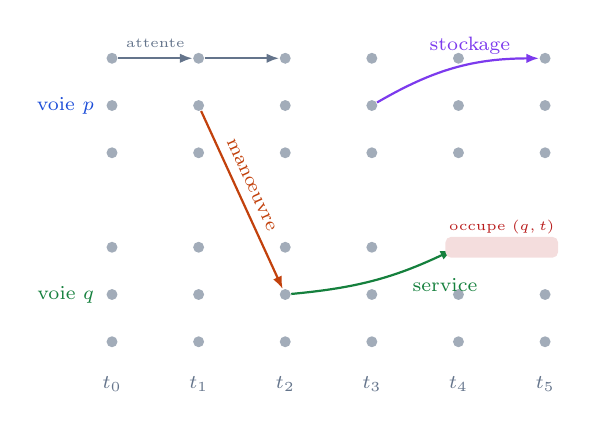
\begin{tikzpicture}[x=1.1cm,y=0.6cm,font=\scriptsize,
        n/.style={circle,fill=mute!60,inner sep=1.4pt},
        a/.style={-{Latex[length=1.6mm]},line width=0.8pt}]
      \foreach \t in {0,...,5} {
        \foreach \l/\yy in {0/5,1/4,2/3} \node[n] (p\l\t) at (\t,\yy) {};
        \foreach \l/\yy in {0/1,1/0,2/-1} \node[n] (q\l\t) at (\t,\yy) {};
        \node[mute] at (\t,-1.9) {$t_{\t}$};
      }
      \node[left=3pt,acc] at (p10) {voie $p$};
      \node[left=3pt,ok] at (q10) {voie $q$};
      \draw[a,mute] (p00) -- node[above,font=\tiny]{attente} (p01); \draw[a,mute] (p01) -- (p02);
      \draw[a,warn] (p11) -- node[above,sloped,pos=0.45]{manœuvre} (q12);
      \draw[a,ok] (q12) to[bend right=10] node[below right=-1pt,pos=0.7]{service} (q04);
      \draw[a,lav] (p13) to[bend left=15] node[above,pos=0.6]{stockage} (p05);
      \fill[bad!15,rounded corners=2pt] ($(q04)+(-0.15,-0.22)$) rectangle ($(q05)+(0.15,0.22)$);
      \node[bad,font=\tiny] at ($(q04)!0.5!(q05)+(0,0.42)$) {occupe $(q,t)$};
    \end{tikzpicture}
    \column{0.43\textwidth}
    \begin{itemize}
      \item \textbf{Nœud} = (voie, instant), pas de temps de 5.
      \item \textbf{Arc} = arrivée, manœuvre, service, stockage, attente, départ, ou \alert{refus}.
      \item \textbf{Chemin} = le planning complet d'un train.
      \item Chaque arc occupe des \textbf{cellules} (voie, instant).
    \end{itemize}
    \medskip
    \begin{block}{Le problème devient}
      Choisir un chemin par train, sans que deux chemins occupent la même cellule.
    \end{block}
  \end{columns}
\end{frame}

% ===================================================================== 4
\begin{frame}{Génération de colonnes}
  \begin{columns}[T,onlytextwidth]
    \column{0.5\textwidth}
    \textbf{Problème maître} : une variable $\lambda_c \in \{0,1\}$ par chemin $c$, de coût $\gamma_c$.
    \begin{align*}
      \min \ & \textstyle\sum_c \gamma_c \lambda_c \\
      \text{s.c.}\ & \textstyle\sum_{c \in \Omega_k} \lambda_c \ge 1 && \forall k \quad (\pi_k)\\
      & \textstyle\sum_{c \ni (r,t)} \lambda_c \le 1 && \forall (r,t) \quad (\mu_{rt})
    \end{align*}
    \vspace{-2pt}
    {\footnotesize (+ une contrainte par service requis)}
    \medskip

    \textbf{Pricing}, pour chaque train $k$ : chercher le chemin de coût réduit minimal
    \[ \bar c = \gamma_c - \pi_k - \textstyle\sum_{(r,t) \in c} \mu_{rt} \]
    \footnotesize = un plus court chemin avec ressources (services faits) dans le graphe.
    \column{0.47\textwidth}
    \centering
    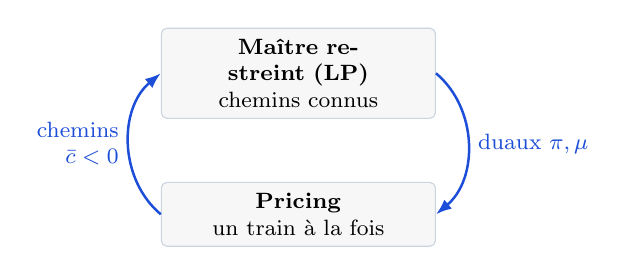
\begin{tikzpicture}[font=\footnotesize,
        bx/.style={draw=line,fill=black!3,rounded corners=2pt,align=center,inner sep=4pt,text width=3.2cm},
        ar/.style={-{Latex[length=2mm]},line width=0.9pt,acc}]
      \node[bx] (m) {\textbf{Maître restreint (LP)}\\ chemins connus};
      \node[bx,below=0.8cm of m] (p) {\textbf{Pricing}\\ un train à la fois};
      \draw[ar] (m.east) to[bend left=50] node[right]{duaux $\pi,\mu$} (p.east);
      \draw[ar] (p.west) to[bend left=50] node[left,align=right]{chemins\\ $\bar c < 0$} (m.west);
    \end{tikzpicture}
    \medskip

    \begin{tikzpicture}
      \begin{axis}[width=\linewidth,height=3.1cm,font=\tiny,
          xlabel={itération},ylabel={valeur du LP},
          ymin=0,ymax=17000,scaled ticks=false,yticklabel style={/pgf/number format/1000 sep={\,}},
          grid=major,grid style={line,opacity=0.5}]
        \addplot[ok,thick,mark=*,mark size=1pt] table[x=it,y=rmp]{data/cg_root_s1.csv};
        \addplot[mute,dashed] coordinates {(0,1959.5) (17,1959.5)};
      \end{axis}
    \end{tikzpicture}\\
    \legende{small 1 : de 16\,040 (tout refusé) à l'optimum LP 1\,959,5 en 18 itérations}
  \end{columns}
\end{frame}

% ===================================================================== 5
\begin{frame}{Branch-and-Price}
  \begin{columns}[T,onlytextwidth]
    \column{0.5\textwidth}
    LP fractionnaire $\Rightarrow$ on \textbf{branche} en interdisant des arcs à un train (le pricing reste exact) :
    \begin{itemize}
      \item \textbf{date d'un service} : avant ou après un instant $t_0$
      \item \textbf{divergence} : au point où les chemins du train se séparent.
    \end{itemize}
    \textbf{Heuristiques primales} tous les 5 nœuds : plongée et MIP sur les colonnes.
    \medskip

    \begin{alertblock}{Limite sur les grandes gares}
      \begin{itemize}
        \item \textbf{6 instances sur 19} sans solution \B\ (medium 3--5, large 2--4)
        \item jusqu'à \textbf{1\,043 s} avant la première solution (small 5).
      \end{itemize}
    \end{alertblock}
    \column{0.47\textwidth}
    \centering
    \shot{width=\linewidth}{img/bp_tree.jpg}\\
    \legende{arbre de branchement rejoué dans l'application\\ (couleur = statut du nœud)}
  \end{columns}
\end{frame}

% ===================================================================== 6
\begin{frame}{Ce que l'IA agentique a apporté au projet}
  \begin{columns}[T,onlytextwidth]
    \column{0.32\textwidth}
    \begin{block}{Comprendre et outiller}
      \footnotesize
      Lecture du solveur C++ existant, instrumentation (itérations, nœuds, bornes, solutions), et \textbf{application de visualisation} (FastAPI, React/D3) d'après notre cahier des charges.
    \end{block}
    \column{0.32\textwidth}
    \begin{exampleblock}{Théoriser l'ALNS}
      \footnotesize
      Idée d'une ALNS réparée par le pricing, théorisée avec l'agent. Il l'a \textbf{rattachée à la littérature} (Ropke \& Pisinger 2006 ; Prescott-Gagnon \emph{et al.} 2009), a vérifié son adéquation au problème, puis l'a \textbf{implémentée} et réglée.
    \end{exampleblock}
    \column{0.32\textwidth}
    \begin{alertblock}{Mesurer et fiabiliser}
      \footnotesize
      Benchmark \B\ / ALNS sur 19 instances, analyse des traces, corrections (bornes négatives, gap affiché à tort à 0\,\%) et une \textbf{erreur de modèle} révélée par l'interface.
    \end{alertblock}
  \end{columns}
  \bigskip

  \begin{columns}[T,onlytextwidth]
    \column{0.48\textwidth}
    \textbf{Notre rôle}\\
    \footnotesize fixer la direction, critiquer les propositions, valider la modélisation, lancer les campagnes sous Gurobi.
    \column{0.48\textwidth}
    \textbf{Le rôle de l'agent}\\
    \footnotesize relier aux méthodes connues, implémenter (C++, Python, TypeScript), tester, mesurer.
  \end{columns}
  \bigskip

  \centering
  \alert{L'agent a surtout raccourci la boucle idée $\to$ implémentation $\to$ mesure.}
\end{frame}

% ===================================================================== 7
\begin{frame}{L'interface : voir les solutions, pas seulement les chiffres}
  \begin{columns}[T,onlytextwidth]
    \column{0.49\textwidth}
    \centering
    \shot{height=2.5cm}{img/sim_s4.jpg}\\
    \legende{\textbf{Simulation} de la gare de $t=0$ à $T$}
    \medskip

    \shot{height=1.8cm}{img/alns_panel.jpg}\\
    \legende{\textbf{Convergence de l'ALNS}}
    \column{0.49\textwidth}
    \centering
    \shot{height=2.5cm}{img/side_maps.jpg}\\
    \legende{\textbf{\B\ et ALNS côte à côte}, même horloge}
    \medskip

    \shot{height=1.8cm}{img/bench_table.jpg}\\
    \legende{\textbf{Benchmark} et export CSV}
  \end{columns}
  \medskip

  \centering
  \small Chaque solution affichée est \textbf{re-vérifiée} à partir des données : c'est ainsi que l'erreur de modèle a été trouvée (bonus).
\end{frame}

% ===================================================================== 8
\begin{frame}{L'ALNS : détruire une partie de la solution, la réparer avec le pricing}
  \begin{columns}[T,onlytextwidth]
    \column{0.52\textwidth}
    \centering
    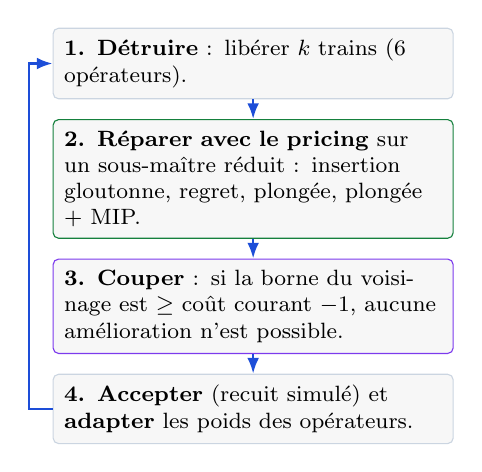
\begin{tikzpicture}[font=\footnotesize,
        bx/.style={draw=line,fill=black!3,rounded corners=2pt,align=left,inner sep=4pt,text width=4.8cm},
        ar/.style={-{Latex[length=2mm]},line width=0.9pt,acc}]
      \node[bx] (d) {\textbf{1. Détruire} : libérer $k$ trains (6 opérateurs).};
      \node[bx,below=0.25cm of d,draw=ok] (r) {\textbf{2. Réparer avec le pricing} sur un sous-maître réduit : insertion gloutonne, regret, plongée, plongée + MIP.};
      \node[bx,below=0.25cm of r,draw=lav] (b) {\textbf{3. Couper} : si la borne du voisinage est $\ge$ \mbox{coût courant $- 1$}, aucune amélioration n'est possible.};
      \node[bx,below=0.25cm of b] (a) {\textbf{4. Accepter} (recuit simulé) et \textbf{adapter} les poids des opérateurs.};
      \draw[ar] (d) -- (r); \draw[ar] (r) -- (b); \draw[ar] (b) -- (a);
      \draw[ar] (a.west) -- ++(-0.3,0) |- (d.west);
    \end{tikzpicture}
    \column{0.45\textwidth}
    \textbf{Pourquoi le pricing}
    \begin{itemize}
      \item Insérer un train = un plus court chemin où les cellules prises sont interdites : on obtient le meilleur chemin \textbf{sans conflit}, en millisecondes.
      \item Mêmes chemins et mêmes duaux que le \B.
      \item La borne évite de chercher là où rien n'est gagnable.
    \end{itemize}
    \medskip

    \textbf{Références}\\
    \scriptsize
    Ropke \& Pisinger, \emph{Transportation Science} 40(4), 2006.\\
    Prescott-Gagnon, Desaulniers \& Rousseau, \emph{Networks} 54(4), 2009.
  \end{columns}
\end{frame}

% ===================================================================== 9
\begin{frame}{Résultats du benchmark : B\&P et ALNS côte à côte}
  \centering
  \scriptsize
  \renewcommand{\arraystretch}{0.86}
  \begin{tabular}{l rrr rrr l}
    \toprule
    & \multicolumn{3}{c}{\textbf{Branch-and-Price}} & \multicolumn{3}{c}{\textbf{ALNS}} & \\
    \cmidrule(lr){2-4}\cmidrule(lr){5-7}
    Instance & coût & écart & 1\textsuperscript{re} sol. & coût & écart & 1\textsuperscript{re} sol. & meilleure \\
    \midrule
      small 1 & 1\,974 & 0,5\,\% & 0,50 s & 1\,974 & 0,5\,\% & < 0,01 s & égalité \\
      small 2 & 12\,457 & 115,6\,\% & 26 s & \win{9\,803} & 69,7\,\% & 0,01 s & \textcolor{ok}{ALNS} \\
      small 3 & 35\,647 & 73,6\,\% & 131 s & \win{28\,662} & 39,5\,\% & 0,02 s & \textcolor{ok}{ALNS} \\
      small 4 & 43\,416 & 56,3\,\% & 142 s & \win{36\,413} & 31,1\,\% & 0,01 s & \textcolor{ok}{ALNS} \\
      small 5 & 80\,500 & 26,1\,\% & 1\,044 s & \win{76\,255} & 19,5\,\% & 0,05 s & \textcolor{ok}{ALNS} \\
      \midrule
      medium 1 & 3\,974 & 0,0\,\% & 9,53 s & 3\,974 & 0,0\,\% & 0,01 s & égalité \\
      medium 2 & 18\,715 & 75,0\,\% & 219 s & \win{16\,053} & 50,1\,\% & 0,02 s & \textcolor{ok}{ALNS} \\
      medium 3 & \multicolumn{3}{c}{\nosol} & \win{35\,852} & 55,4\,\% & 0,08 s & \textcolor{ok}{ALNS seule} \\
      medium 4 & \multicolumn{3}{c}{\nosol} & \win{101\,814} & 26,3\,\% & 0,33 s & \textcolor{ok}{ALNS seule} \\
      medium 5 & \multicolumn{3}{c}{\nosol} & \win{182\,983} & 58,3\,\% & 0,54 s & \textcolor{ok}{ALNS seule} \\
      \midrule
      large 1 & 7\,264 & 0,0\,\% & 24 s & 7\,264 & 0,0\,\% & 0,03 s & égalité \\
      large 2 & \multicolumn{3}{c}{\nosol} & \win{26\,139} & 28,7\,\% & 0,15 s & \textcolor{ok}{ALNS seule} \\
      large 3 & \multicolumn{3}{c}{\nosol} & \win{79\,313} & 150,2\,\% & 0,45 s & \textcolor{ok}{ALNS seule} \\
      large 4 & \multicolumn{3}{c}{\nosol} & \win{220\,636} & 225,1\,\% & 0,77 s & \textcolor{ok}{ALNS seule} \\
      \midrule
      variant 1 & 2\,475 & 3,8\,\% & 1,30 s & \win{2\,471} & 3,7\,\% & < 0,01 s & \textcolor{ok}{ALNS} \\
      variant 2 & 12\,078 & 101,6\,\% & 39 s & \win{11\,338} & 89,2\,\% & 0,01 s & \textcolor{ok}{ALNS} \\
      variant 3 & 28\,787 & 21,7\,\% & 28 s & \win{28\,624} & 21,1\,\% & 0,03 s & \textcolor{ok}{ALNS} \\
      variant 4 & 53\,119 & 12,9\,\% & 714 s & \win{52\,998} & 12,6\,\% & 0,14 s & \textcolor{ok}{ALNS} \\
      variant 5 & 84\,923 & 15,7\,\% & 163 s & \win{79\,501} & 8,3\,\% & 0,31 s & \textcolor{ok}{ALNS} \\
    \bottomrule
  \end{tabular}\\[3pt]
  \raggedright
  {\scriptsize\mdseries\color{mute} En vert : la moins chère. Écart à la meilleure borne connue (0\,\% = optimum prouvé). Gurobi, runs de 400 à 1\,250 s.}
\end{frame}

% ===================================================================== 10
\begin{frame}{Conclusion et perspectives}
  \begin{columns}[T,onlytextwidth]
    \column{0.32\textwidth}
    \begin{exampleblock}{Bilan}
      \footnotesize
      \begin{itemize}
        \item un \B\ corrigé et observable
        \item une ALNS fondée sur le pricing : solution en moins d'une seconde, meilleure sur 10 instances sur 13
        \item une interface qui a révélé une erreur de modèle.
      \end{itemize}
    \end{exampleblock}
    \column{0.32\textwidth}
    \begin{alertblock}{Limites}
      \footnotesize
      \begin{itemize}
        \item écarts de 29 à 225\,\% sur les grandes gares : borne de racine faible
        \item l'ALNS ne prouve rien seule
        \item durées de run pas toujours égales.
      \end{itemize}
    \end{alertblock}
    \column{0.32\textwidth}
    \begin{block}{Perspectives}
      \footnotesize
      \begin{itemize}
        \item l'ALNS comme heuristique \emph{dans} le \B
        \item strong branching, stabilisation des duaux
        \item réglage de l'ALNS (racine, recuit, diversité des opérateurs).
      \end{itemize}
    \end{block}
  \end{columns}
  \bigskip

  \centering
  \alert{Méthode exacte et heuristique partagent le même moteur : graphe, pricing, borne.}
\end{frame}

% ===================================================================== bonus
\appendix
\begin{frame}{Bonus : deux trains se croisaient sur la même voie}
  \begin{columns}[T,onlytextwidth]
    \column{0.36\textwidth}
    \textbf{1. Vu dans la simulation}\\[2pt]
    \shot{width=0.9\linewidth}{img/user_crossing.jpg}\\
    \footnotesize T3 et T11 avancent l'un vers l'autre sur la même voie, au même pas de temps.
    \medskip

    \textbf{2. Pourquoi c'était permis}\\[2pt]
    \scriptsize
    \begin{tabular}{lcc}
      \toprule
      & $t$ & $t+5$ \\
      \midrule
      A : $p\to q$ & $p$ & $q$ \\
      B : $q\to p$ & $q$ & $p$ \\
      lien $p$--$q$ & \multicolumn{2}{c}{\color{bad}\bfseries jamais occupé} \\
      \bottomrule
    \end{tabular}\\[2pt]
    Une manœuvre n'occupait que sa voie de départ.
    \column{0.6\textwidth}
    \textbf{3. Mesuré par l'application}\\[2pt]
    \centering\shot{height=2cm}{img/crossing_alert.jpg}\\
    \raggedright\legende{89 croisements dans les 10 solutions Gurobi du modèle d'origine}
    \medskip

    \textbf{4. Corrigé} : chaque lien $\ell$ devient une ressource de capacité 1, dans les deux sens :
    \[ \textstyle\sum_{c \text{ utilise } \ell \text{ à } \tau} \lambda_c \le 1 \qquad \forall \ell,\ \forall \tau \]
    \footnotesize
    \begin{itemize}
      \item 0 croisement après correction
      \item pricing inchangé : 66\,548 coûts réduits recalculés, 0 écart
      \item borne de racine inchangée sur les petites instances.
    \end{itemize}
  \end{columns}
\end{frame}

\end{document}
